\begin{figure}[htbp]
    \centering
    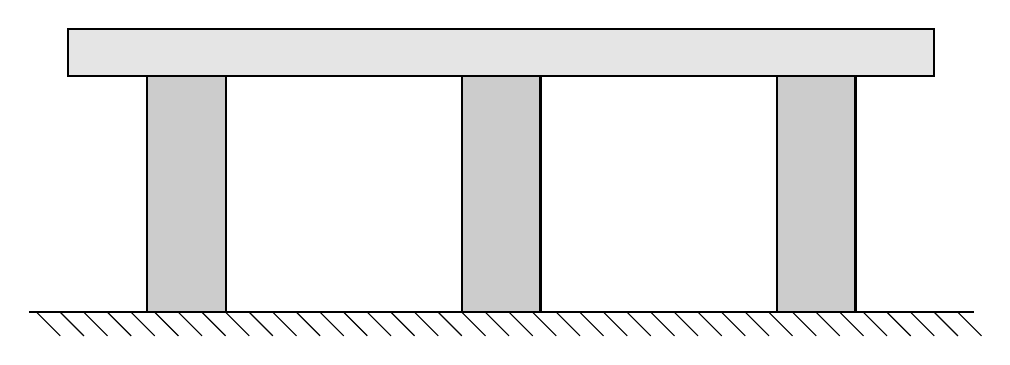
\begin{tikzpicture}[scale=1]
        % Beam
        \draw[fill=gray!20, thick] (0,3) rectangle (11,3.6);

        % Pillars
        \foreach \x in {1, 5, 9} {
            \draw[fill=gray!40, thick] (\x,0) rectangle (\x+1,3);
        }

        % Ground line
        \draw[thick] (-0.5,0) -- (11.5,0);

        % Ground hatching
        \foreach \x in {-0.4,-0.1,...,11.4} {
            \draw (\x,0) -- (\x+0.3,-0.3);
        }
    \end{tikzpicture}
    \caption{Beam resting on three pillars.}
    \label{fig:beam-three-pillars}
\end{figure}
